\documentclass[11pt]{article}
\usepackage{amsmath,amssymb,amsthm}
\usepackage{mathtools}
\usepackage{geometry}
\usepackage[hypertexnames=false]{hyperref}
\usepackage{enumitem}
\usepackage{tikz}
\usepackage{float}
\usetikzlibrary{calc}
\usetikzlibrary{positioning}
\usetikzlibrary{decorations.pathreplacing}
\geometry{margin=1in}

\newtheorem{theorem}{Theorem}[section]
\newtheorem{definition}{Definition}[section]
\newtheorem{lemma}{Lemma}[section]
\newtheorem{proposition}{Proposition}[section]
\newtheorem{corollary}{Corollary}[section]
\newtheorem{remark}{Remark}[section]

\title{The Catalan Light Cone:\\
Dyck Paths as a Discrete Substrate for Causal Geometry, Quantum Amplitudes, and Computation}
\author{Paul Fernandez}
\date{}

\begin{document}
\maketitle

\begin{abstract}
\noindent
We study the Catalan family of structures---Dyck paths, full binary trees, and
balanced parenthesis expressions---as a single discrete space of admissible
histories with multiple equivalent ``coordinate systems.'' The Dyck constraint
induces a natural causal prefix order, and organizing histories by tier and
lateral spread yields a discrete cone whose extremal configurations reproduce a
light-cone--like causal envelope.

Classical results on conditioned random walks imply that, under diffusive
scaling, Dyck ensembles converge to Brownian excursions. This provides a
continuum comparison in which the induced evolution is governed by the heat
operator on the half-line (with the Dyck conditioning encoded by boundary
conditions, or equivalently by conditioning), and under analytic continuation one
obtains the free Schr\"odinger equation.

The same Catalan shapes also serve as unlabeled application skeletons for
$\lambda$-calculus and SKI terms (after choosing a standard finite encoding of
symbols). Under this reading, causal extension aligns with functional
application while local collapse aligns with computational reduction. We also
present a minimal amplitude construction: given an observable/coarse-graining
$f$ and an additive phase functional (e.g.\ Dyck area), coherent summation over
the preimages $f^{-1}(x)$ produces interference under Born-style squaring.

Throughout, we distinguish rigorously established statements (combinatorics,
scaling limits, and commutation of disjoint local rewrites) from interpretive or
open extensions (measurement, interactions, constants).
\end{abstract}

\section{Introduction}
Discrete approaches to fundamental physics suggest that continuum
spacetime and quantum dynamics may emerge from deeper combinatorial structure.
Examples include causal sets \cite{bombelli87}, discrete random surfaces and
Causal Dynamical Triangulations (CDT) \cite{ambjorn01,ambjorn12}, spin
networks and loop quantum gravity \cite{rovelli04}, tensor networks
\cite{orus14}, and rewriting systems inspired by $\lambda$-calculus and
combinatory logic.

Typically, however, these models require multiple independent ingredients: a
relation or graph for causal structure, an algebra for computation, and
additional rules for quantum propagation. This work explores a more economical
possibility: that a \emph{single} recursive structure simultaneously supports
all three.

The focus is the \emph{Catalan substrate}, the family of structures counted by
the Catalan numbers \cite{stanley-catalan}, including Dyck paths, full binary
trees, and balanced parenthesis expressions. These objects are usually studied
in enumerative combinatorics, probability theory, and theoretical computer
science. Here they are treated instead as a space of \emph{admissible
histories} generated by a minimal growth constraint.

\paragraph{One object, three coordinate systems.}
We will move freely between three canonically bijective Catalan families:
\begin{itemize}
  \item Dyck paths (a constrained nearest-neighbour walk),
  \item full binary trees (recursive branching structure),
  \item parenthesis/pairs encodings (a linear trace of the same tree).
\end{itemize}
Switching between these views is not a simulation; it is a change of
representation of the same underlying object. Each view foregrounds different
structure: Dyck paths make causal order and scaling limits transparent; trees
make locality and computation transparent; and pairs encodings make uniform
syntax convenient.

\paragraph{Contributions and scope.}
The paper isolates a common structural core shared by three domains:
\begin{enumerate}[label=(\roman*)]
	\item \textbf{Causal geometry:} the prefix order on Dyck prefixes induces a
		discrete causal structure and a cone-shaped envelope with sharp extremals.
	\item \textbf{Continuum comparison:} classical conditioned-walk results yield a
		diffusion limit (Brownian excursion, heat equation on the half-line), and an
		analytic-continuation bridge to the free Schr\"odinger equation
		\cite{le-gall05,janson07,feynman-hibbs65,kac49}.
		\item \textbf{Computation:} Catalan tree shapes provide unlabeled application
			skeletons for standard Turing-complete functional calculi (after choosing a
			finite encoding of symbols), and local reductions remain internal to the same
			family \cite{church33,CurryFeys1958,barendregt84}.
	\item \textbf{Amplitudes:} given a coarse-graining (observable) and an additive
		phase functional, coherent summation over indistinguishable histories produces
		interference under Born-style squaring.
\end{enumerate}
We do not attempt to derive interactions, constants, or a unique measurement
postulate; where additional structure is introduced (e.g.\ complex phases and
Born-style probabilities), it is presented as a minimal construction layered on
the Catalan kinematics.

\paragraph{Organization.}
Section~\ref{sec:catalan_cone} establishes the discrete causal geometry of the
Catalan lattice and its interpretation as a light cone. Section~\ref{sec:computation}
develops the computational correspondence via binary application trees and pairs
encodings. Section~\ref{sec:amplitudes} introduces a minimal amplitude
construction and the continuum comparison to diffusion and Schr\"odinger
dynamics.%
\footnote{Depending on reader background, Sections~\ref{sec:computation} and
Section~\ref{sec:amplitudes} may be read in either order after the geometric
setup in Section~\ref{sec:catalan_cone}.}
Locality and disjoint-commutation are discussed in Section~\ref{sec:locality}.
Optional coordinate embeddings, technical notes, and illustrative examples are
collected in appendices, separate from the main formal development.

\section{The Catalan Light Cone as a Discrete Causal Geometry}
\label{sec:catalan_cone}

\subsection{Dyck paths and growth tiers}
A Dyck path of semilength $n$ is a walk on the integers satisfying
\[
	H_{k+1} = H_k \pm 1, \qquad H_k \ge 0, \qquad H_0 = H_{2n} = 0.
\]
Equivalently, Dyck paths are balanced parenthesis strings or full binary trees
with $n$ internal nodes. The number of such paths is the $n$th Catalan number
\[
	C_n = \frac{1}{n+1}\binom{2n}{n}.
\]
Each up--down pair \(()\) represents a minimal unit of growth. The integer $n$
will be called the \emph{tier} and will be interpreted as a discrete proper
time.

\subsection{Prefix order and causality}
Let $\mathcal{C}$ denote the set of \emph{Dyck prefixes}: balanced-parentheses
prefixes that never go below height $0$. Define a partial order by extension:
$u\preceq v$ iff $u$ is a prefix of $v$. We interpret this order as a causal
relation: $u\preceq v$ means that $u$ lies in the causal past of $v$, while
prefixes that diverge represent incompatible futures. This prefix order defines
a discrete causal structure:
\begin{itemize}
	\item every node has a unique causal past,
	\item multiple incompatible futures may branch from the same prefix,
	\item cycles are prohibited by construction.
\end{itemize}
No additional causal axiom is introduced; causality is enforced combinatorially
by the Dyck constraint.

\subsection{Extremal configurations: chain and star}
At fixed tier $n$ there are many Dyck paths. Two extremal configurations play a
distinguished role:
\begin{itemize}
	\item the \emph{chain} (or spine)
		\[
			(((\cdots))),
		\]
		fully nested, with maximal depth and minimal spread;
	\item the \emph{star}
		\[
			()()()\cdots(),
		\]
		fully separated, with minimal depth and maximal spread.
\end{itemize}
All other configurations interpolate between these extremes. Together, the set
of Dyck paths at tier $n$ forms a discrete envelope bounded by the chain and
the star.

\begin{figure}[h]
	\centering
	% Placeholder: schematic light-cone diagram
	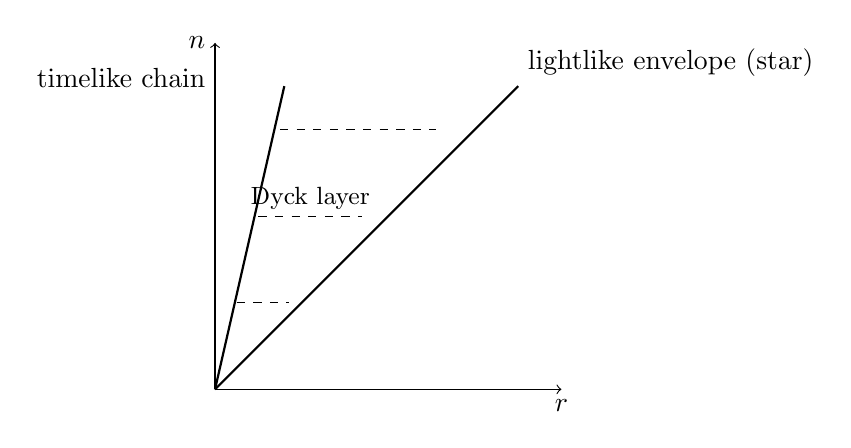
\begin{tikzpicture}[scale=1.1]
		% axes
			\draw[->] (0,0) -- (0,4) node[left] {$n$};
			\draw[->] (0,0) -- (4,0) node[below] {$r$};
		% cone boundaries
		\draw[thick] (0,0) -- (3.5,3.5);
		\draw[thick] (0,0) -- (0.8,3.5);
		% discrete layers
		\foreach \y in {1,2,3} {
			\draw[dashed] (0.25*\y,\y) -- (0.85*\y,\y);
		}
		% labels
		\node[left] at (0,3.6) {timelike chain};
		\node[above right] at (3.5,3.5) {lightlike envelope (star)};
		\node at (1.1,2.2) {\small Dyck layer};
		\end{tikzpicture}
		\caption{The Catalan light cone.
			Tier $n$ (the number of Dyck units) plays the role of proper time, while
			breadth $r$ measures spatial radius. All Dyck configurations at fixed tier
			lie between the fully nested chain (timelike extreme) and the fully separated
			star (lightlike envelope).
			Discrete Dyck layers approximate constant-time hypersurfaces, and the bound
		$r \le n$ is enforced combinatorially.}
		\label{fig:catalan-cone}
\end{figure}

\subsection{Breadth as spatial extent}
Define the \emph{breadth} $r(w)$ of a Dyck path $w$ to be the size of a
largest level set in the associated full binary tree:
\[
	r(w) := \max_{\ell} \{\text{number of nodes at depth } \ell\}.
\]
Equivalently, $r(w)$ is the maximal number of non-overlapping pairs at a common
nesting depth. For a Dyck word of tier $n$ there are $n$ matched pairs in
total, so
\[
	1 \le r(w) \le n,
\]
with $r=1$ for the fully nested chain and $r=n$ for the fully separated star.
The inequality
\[
	r \le n
\]
is enforced purely by the recursive constraint. It is the discrete analogue of
the relativistic light-cone bound $|\Delta x| \le \Delta t$ (in units with
$c=1$).

\subsection{Depth--breadth tradeoff}
Let $h(w)$ denote the maximum height of a Dyck path, i.e.\ the maximum nesting
depth of its associated full binary tree (root at depth $0$). Recall that the
breadth $r(w)$ is the maximum number of nodes occurring at any fixed depth
level:
\[
r(w):=\max_{\ell}{\text{number of nodes at depth }\ell}.
\]
Depth and breadth are not independent. In any full binary tree, the number of
nodes at depth $\ell$ is at most $2^{\ell}$ (each level can at most double from
its parent level). Hence, if the maximum level set size $r(w)$ occurs at depth
$\ell_\ast$, then
\[
r(w)\le 2^{\ell_\ast}\le 2^{h(w)}
\quad\Rightarrow\quad
h(w)\ge \log_2 r(w).
\]
Thus configurations with large breadth necessarily have logarithmically large
depth. Equivalently, very shallow trees cannot support wide level sets, while
trees with very large depth must concentrate most nodes away from any single
breadth-maximizing level.

\begin{remark}[Kraft equality for leaf depths]
For the full binary tree associated to a Dyck path, if $L$ is the set of leaves
and $d(\ell)$ denotes the depth of $\ell\in L$ (root at depth $0$), then
\[
\sum_{\ell\in L} 2^{-d(\ell)} = 1.
\]
Equivalently, the leaf depths form a complete binary prefix code. This gives a
global constraint on allowable depth profiles beyond the crude level bound
$r(w)\le 2^{h(w)}$; see \cite{cover-thomas}.
\end{remark}

\begin{figure}[h]
		\centering
		\[
			\begin{array}{ccl}
			((())) & \quad & (h=3,\ r=1) \\
			(()()) &      & (h=2,\ r=2) \\
			(())() &      & (h=2,\ r=2) \\
			()(()) &      & (h=2,\ r=2) \\
			()()() &      & (h=1,\ r=3)
		\end{array}
	\]
	\caption{All Dyck words of tier $n=3$, ordered from maximal nesting (chain)
		to maximal separation (star). These five configurations exhaust the discrete
		causal possibilities at fixed proper time.
		Depth $h$ and breadth $r$ interpolate between the two extremes, illustrating
		the intrinsic tradeoff enforced by the Dyck constraint.
	Higher tiers replicate this structure at larger scale.}
	\label{fig:dyck-n3}
\end{figure}

\subsection{Cone structure}
Organizing Dyck paths by tier $n$ and breadth $r$ yields a discrete cone:
\begin{itemize}
	\item each tier is a ``constant-time'' slice,
	\item the chain defines the timelike axis,
	\item the star defines the lightlike boundary,
	\item admissible configurations fill the interior.
\end{itemize}
This structure will be referred to as the \emph{Catalan light cone}.

\subsection{Scaling behavior}
Classical results on conditioned random walks show that typical Dyck paths at
tier $n$ have height and breadth of order $\sqrt{n}$
\cite{le-gall05,janson07,addario-berry13}. Extremal configurations saturate
the linear bound $r\le n$, while typical configurations lie deep within the
cone. This separation between extremal and typical behavior mirrors the role of
null, timelike, and spacelike trajectories in relativistic geometry.

\begin{theorem}[Discrete light-cone bound and scaling]
	Let $w$ be a Dyck word of semilength $n$ and breadth $r(w)$ as above. Then
	\[
		1 \le r(w) \le n.
	\]
	Moreover, for a uniformly random Dyck word of semilength $n$, the typical
	height and breadth are of order $\sqrt{n}$.
\end{theorem}
\noindent
The first statement follows from the definition of $r(w)$ and the fact that
there are $n$ internal nodes, while the scaling behavior is a consequence of
invariance-principle results for conditioned random walks
\cite{le-gall05,janson07,addario-berry13}.

\paragraph{Coordinate charts and continuum comparisons.}
Appendix~\ref{appendix:coordinate-charts} collects optional coordinate-chart
constructions (null-count embeddings and related continuum comparisons) used for
intuition; the combinatorial results below do not depend on these embeddings.

\subsection{Recursive Self-Similarity and Local Re-Centering}
\label{sec:selfsimilarity}

A key structural property of the Catalan substrate is its \emph{recursive
self-similarity}. Every Dyck word may be viewed as a node in the infinite
prefix tree of admissible Dyck prefixes. At any such node $u$, with current
height $h$ and remaining length budget sufficient to return to height~$0$, the
set of all admissible continuations of $u$ forms a subtree whose shape is
determined entirely by $h$. This subtree is canonically isomorphic to the
Dyck-prefix tree that begins at height $h$ rather than at height $0$.

Formally, let $\mathcal{C}$ denote the Dyck-prefix tree (the poset of Dyck
prefixes under extension) and
$\mathcal{C}_h$ denotes the Dyck-prefix tree conditioned to start at height $h$
(i.e.\ with $H_0=h$ and $H_k\ge 0$ for all $k$), then for every prefix $u$ of
height $h$ we have a canonical isomorphism

\[
	\mathcal{C}(u) \;\cong\; \mathcal{C}_h.
\]

Thus every node of the global Catalan possibility tree is the root of a scaled
copy of the entire admissible-future structure, with scaling determined solely
by local height. The recursive decomposition of full binary trees,

\[
	T = \bullet(T_L,T_R),
\]

makes the same fact explicit in the tree representation: each subtree of a
Catalan tree is itself a Catalan tree, and the decomposition applies inductively
at every depth.

This recursive self-similarity has two important consequences for the geometric
interpretation developed in this paper:

\begin{enumerate}[label=(\roman*)]
	\item \textbf{Locality and re-centering.}
		Because the admissible future of any prefix depends only on its present
		height, not on its global position, the Catalan light-cone geometry is
		\emph{locally homogeneous}. The causal cone may be re-centered at any node
		without altering its shape: moving the focus does not change the structure of
		admissible futures, only the value of the local height at which the cone is
		rooted.

	\item \textbf{Scale invariance of the substrate.}
		The same recursive rules govern growth at every depth. The local possibility
		space looks the same at all scales, in the sense that the subtree below any
		node is again Catalan. This is the combinatorial source of the invariance
		principles (Dyck $\to$ Brownian excursion) appearing in the continuum limit.
\end{enumerate}

In summary, the Catalan substrate is self-similar at every node: each point in
the possibility space contains a full Catalan future scaled by its current
height. This allows the causal and geometric analysis of later sections to be
performed relative to \emph{any} node of the prefix tree. The light cone is not
anchored to a global origin; it is an intrinsic, relocatable geometric feature
of the recursive structure itself.

\subsection{Multiple Local Cones and Relational Geometry}
\label{sec:multiplecones}

The same prefix order that defines causality also yields a family of \emph{local
cones}: every Dyck prefix $u\in\mathcal{C}$ induces a future $\mathcal{C}(u)$ of
admissible extensions, i.e.\ the same growth law re-centered at $u$.
Two prefixes $u$ and $v$ relate in exactly two ways:
\begin{enumerate}[label=(\roman*)]
	\item \textbf{Nested cones.} If $u\preceq v$, then $\mathcal{C}(v)\subseteq \mathcal{C}(u)$.
	\item \textbf{Divergent cones.} If neither prefix contains the other, then $u$
		and $v$ share a maximal common prefix $w$ and have disjoint futures beyond $w$.
\end{enumerate}

Thus the cone picture is relocatable: it appears at every node, cones nest along
causal chains, and branching produces incompatible futures.

\begin{figure}[h]
	\centering
	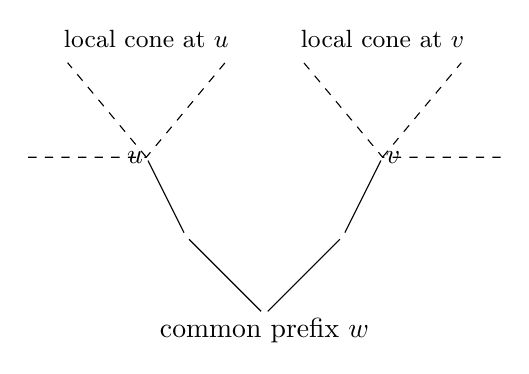
\begin{tikzpicture}[scale=1.0, every node/.style={inner sep=1pt}]
		% Common causal past
		\node (root) at (0,0) {};
		\node (a1)   at (-1,1) {};
		\node (b1)   at (1,1) {};

		% Two divergent prefixes u and v
		\node (u) at (-1.5,2) {};
		\node (v) at (1.5,2) {};

		% Subcones below u
		\draw[dashed] (-3,2) -- (-1.5,2) -- (-0.5,3.2);
		\draw[dashed] (-1.5,2) -- (-2.5,3.2);

		% Subcones below v
		\draw[dashed] (3,2) -- (1.5,2) -- (0.5,3.2);
		\draw[dashed] (1.5,2) -- (2.5,3.2);

		% Edges in prefix tree
		\draw (root) -- (a1);
		\draw (root) -- (b1);
		\draw (a1) -- (u);
		\draw (b1) -- (v);

		% Labels
		\node[left]  at (-1.5,2) {$u$};
		\node[right] at (1.5,2) {$v$};
		\node[below] at (0,0) {common prefix $w$};

		\node at (-1.5,3.5) {\small local cone at $u$};
		\node at (1.5,3.5) {\small local cone at $v$};
	\end{tikzpicture}
		\caption{Two Dyck prefixes $u$ and $v$ diverging from a shared ancestor $w$.
			Dashed regions indicate the local Catalan cones rooted at $u$ and $v$.
			Cones nest along causal chains and diverge after branching points, producing
		a family of local, relocatable causal geometries on the Catalan substrate.}
	\label{fig:multiple-cones}
\end{figure}

\subsection{Summary}
The Catalan substrate supports a discrete causal geometry determined entirely
by recursive constraint. Without introducing a manifold, metric, or causal
relation by fiat, it yields:
\begin{itemize}
	\item a partial order interpretable as causality,
	\item a cone-shaped causal envelope,
	\item intrinsic bounds on spatial extension,
	\item well-defined constant-time layers.
\end{itemize}
Subsequent sections place dynamical rules---quantum amplitudes and
computational reduction---on this geometry.

\section{Recursive Pairing and Universal Computation}
\label{sec:computation}

\noindent
We now read the same Catalan objects from the computational side. Full binary
trees serve as application frames, while pairs encodings provide a uniform
parenthesis-only syntax. The only additional choice needed to represent concrete
programs is an encoding of symbols at leaves.

\subsection{Pairs expansion}

\paragraph{Catalan shapes as program frames.}

The Catalan family---Dyck paths, full binary trees, and balanced-parenthesis
expressions---forms the free magma on a single binary constructor: it is the
space of all finite binary application frames. As observed in classical
treatments of the $\lambda$-calculus and combinatory logic
\cite{CurryFeys1958,barendregt84}, application is binary, so every SKI term (and
every $\lambda$-term after fixing a binding convention) has a canonical
representation as a finite binary application tree: internal nodes encode
application; leaves encode atomic symbols (variables, constants, or combinators).
Conversely, any finite binary tree equipped with leaf labels denotes a unique
applicative term over that alphabet, modulo surface syntax. Since SKI is
computationally universal, this yields an explicit embedding of all computable
programs (as terms) within the Catalan substrate. The apparent choice of leaf
alphabet can itself be internalized by representing symbols as distinguished
Catalan motifs (Remark~\ref{rem:symbol-motifs}).

\begin{remark}[Symbols as Distinguished Motifs]
\label{rem:symbol-motifs}
Although we sometimes describe leaf labels as an external choice, one may work
in a purely structural setting: there is an injective encoding of labeled
application trees (and in particular SKI terms) into unlabeled Catalan trees by
tagging constructor nodes and representing each symbol by a fixed subtree motif.
See Lemma~\ref{lem:symbol-motifs} in Appendix~\ref{appendix:computational-foundations}.
\end{remark}

This observation also extends to operational semantics. Standard reductions
(such as $\beta$-reduction or SKI contraction) are local rewrite rules on binary
trees, and the pairs-expansions of combinators remain within the Catalan family.
Accordingly, a program, its intermediate expansion frames, and each permissible
reduction schedule are all representable as paths through a single Catalan
substrate. Selecting a program shape or selecting a specific reduction history
is therefore equivalent to selecting a path in the Catalan tree. In this sense
the Catalan substrate uniformly encodes program syntax, program semantics, and
the full ensemble of admissible computational histories.

	\begin{proposition}[Catalan Universality for Program Structure]
		\label{prop:catalan-programs}
		Let $\mathcal{C}$ denote the Catalan family of finite full binary trees.
		Every program in any Turing-complete functional calculus (such as the
		$\lambda$-calculus or SKI) admits a canonical representation as an element of
		$\mathcal{C}$ with leaf labels drawn from a finite alphabet (after fixing a
		standard encoding of symbols). Conversely,
		every labeled element of $\mathcal{C}$ denotes a unique program modulo surface
		syntax. Furthermore, standard operational semantics (including
		$\beta$-reduction and SKI contraction) act as local rewrite rules that
		preserve membership in $\mathcal{C}$. Thus a program, its syntactic
	expansions, and every admissible reduction history correspond to paths within
	the Catalan substrate.
\end{proposition}
\noindent
A proof sketch is provided in
Appendix~\ref{appendix:computational-foundations}.

\paragraph{Two canonical parenthesis encodings.}
There are (at least) two particularly useful parenthesis-only encodings of a
full binary tree:

\begin{itemize}
  \item \textbf{Dyck encoding} (``walk'' view): balanced parentheses of length
    $2n$, naturally adapted to height profiles and scaling limits.
  \item \textbf{Pairs (S-expression) encoding} (``cons'' view): write each leaf
    as \texttt{()} and each internal node as a parenthesized pair of its two
    children, i.e.\ $T=(L,R)\mapsto (\texttt{enc}(L)\,\texttt{enc}(R))$.  This is
    a variable- and label-free Lisp-style representation with \texttt{()} as the
    only atom.
\end{itemize}

In particular, in the \emph{pairs} encoding, the smallest object is the empty
pair \texttt{()}, and the smallest nontrivial \emph{binary} object is
\texttt{(()())}, i.e.\ a root pair whose two children are leaves.  In the Dyck
encoding, the semilength-$1$ object is \texttt{()}, since Dyck words begin only
after the first matched pair exists.

\subsection{A small tier shown three ways (Dyck / tree / pairs)}
Figure~\ref{fig:trees-n3-tikz} augments the standard Dyck-$n=3$ list by
displaying, for the \emph{same} five Catalan shapes, the corresponding pairs
(S-expression) encodings.

\begin{figure}[H]
  \centering
  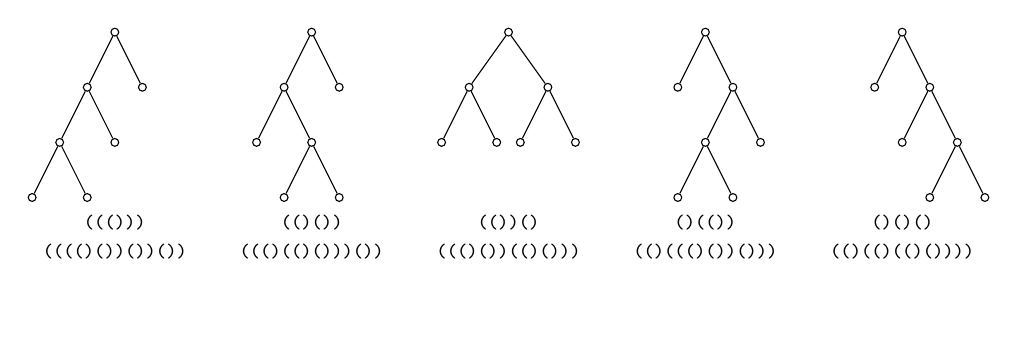
\begin{tikzpicture}[
    level 1/.style={level distance=7mm,sibling distance=7mm},
    level 2/.style={level distance=7mm,sibling distance=7mm},
    every node/.style={circle,draw,inner sep=1pt,minimum size=2pt}
    ]
    % Order: ((())), (()()), (())(), ()(()), ()()()
    % Pairs encodings (canonical): 
    % ((())) -> (((()())())())
    % (()()) -> ((()(()()))())
    % (())() -> ((()())(()()))
    % ()(()) -> (()((()())()))
    % ()()() -> (()(()(()())))
    %
    % 1) ((()))
    \begin{scope}[shift={(-5,0)}]
      \node {}
        child { node {}
          child { node {}
            child { node {} }
            child { node {} }
          }
          child { node {} }
        }
        child { node {} };
      \node[draw=none,align=center] at (0,-2.6)
      {\scriptsize\texttt{((()))}\\[-0.6mm]\scriptsize\texttt{(((()())())())}};
    \end{scope}
    % 2) (()())
    \begin{scope}[shift={(-2.5,0)}]
      \node {}
        child { node {}
          child { node {} }
          child { node {}
            child { node {} }
            child { node {} }
          }
        }
        child { node {} };
      \node[draw=none,align=center] at (0,-2.6)
      {\scriptsize\texttt{(()())}\\[-0.6mm]\scriptsize\texttt{((()(()()))())}};
    \end{scope}
    % 3) (())()
    \begin{scope}[
      shift={(0,0)},
      level 1/.style={level distance=7mm,sibling distance=10mm}
      ]
      \node {}
        child { node {}
          child { node {} }
          child { node {} }
        }
        child { node {}
          child { node {} }
          child { node {} }
        };
      \node[draw=none,align=center] at (0,-2.6)
      {\scriptsize\texttt{(())()}\\[-0.6mm]\scriptsize\texttt{((()())(()()))}};
    \end{scope}
    % 4) ()(())
    \begin{scope}[shift={(2.5,0)}]
      \node {}
        child { node {} }
        child { node {}
          child { node {}
            child { node {} }
            child { node {} }
          }
          child { node {} }
        };
      \node[draw=none,align=center] at (0,-2.6)
      {\scriptsize\texttt{()(())}\\[-0.6mm]\scriptsize\texttt{(()((()())()))}};
    \end{scope}
    % 5) ()()()
    \begin{scope}[shift={(5,0)}]
      \node {}
        child { node {} }
        child { node {}
          child { node {} }
          child { node {}
            child { node {} }
            child { node {} }
          }
        };
      \node[draw=none,align=center] at (0,-2.6)
      {\scriptsize\texttt{()()()}\\[-0.6mm]\scriptsize\texttt{(()(()(()())))}};    
    \end{scope}
  \end{tikzpicture}
  \vspace{-2.5em}
  \caption{The five Catalan shapes at tier $n=3$ shown as (i) Dyck words,
  (ii) full binary trees, and (iii) pairs (S-expression) encodings in which each
  leaf is \texttt{()} and each internal node is a parenthesized pair of its two
  children (as if one were looking "down into" the tree). These are three
  coordinate systems for the same underlying Catalan objects.}
  \label{fig:trees-n3-tikz}
\end{figure}

\subsection{Connection to \texorpdfstring{$\lambda$}{lambda}-calculus and SKI}

Full binary trees are a standard representation of SKI terms, and they capture
the application skeleton of $\lambda$-terms \cite{church33,CurryFeys1958,barendregt84}.
A full $\lambda$-encoding requires a binding convention (e.g.\ variables as leaf
labels or positions, and abstraction as a structural marker), while application
is encoded by the tree's binary node. Under the pairs expansion, each Dyck tree canonically determines an
unlabeled application graph. When variables are suppressed, the resulting graphs
coincide with the structure graphs used in combinatory logic. No additional
primitives beyond recursive pairing are required to obtain this representation.

Choosing a finite set of tree patterns to represent the SKI combinators and
interpreting local tree rewrites as SKI reduction therefore equips the Catalan
substrate with a standard universal calculus: every partial recursive function
can be encoded as an SKI term \cite{CurryFeys1958,barendregt84}, and hence by a
finite Dyck tree, and every computation corresponds to a sequence of local tree
transformations. In this
sense, the Catalan substrate is \emph{computationally universal}. What is new
here is that the same underlying objects simultaneously carry a causal and
geometric interpretation.

\subsection{Reduction and local collapse}

In the computational interpretation, reduction corresponds to local pattern
replacement. A redex occupies a finite region of a tree and may be reduced
without reference to distant subtrees. This locality mirrors the causal
structure established in Section~\ref{sec:catalan_cone}. From the perspective
of the Catalan lattice, reduction may be viewed as \emph{collapse}: a locally
ambiguous structure is replaced by a simpler one consistent with the global
constraint. Importantly, collapse does not alter causal ancestry; it refines an
already-admissible history. For standard calculi (e.g.\ $\lambda$/SKI),
confluence ensures uniqueness of normal forms when they exist, and more locally
reductions supported on disjoint subtrees commute. This computational fact will
later support an interpretation of spacelike commutativity.

\subsection{Summary}

Recursive pairing suffices to encode universal computation. Via the pairs
expansion, Dyck trees and application graphs are two views of the same
structure. Local computational reduction aligns naturally with causal locality
on the Catalan light cone.

\section{Quantum Amplitudes on the Catalan Lattice}
\label{sec:amplitudes}

\noindent
This section layers a minimal amplitude calculus on the Catalan history space.
The key inputs are (i) a coarse-graining/observable $f$ identifying which
histories are regarded as the same outcome, and (ii) a choice of additive phase
functional on histories. Given these, we define amplitudes by coherent summation
over preimages and probabilities by normalized squared magnitudes, in analogy
with the Born rule \cite{feynman-hibbs65}.

\subsection{Histories as paths}

Interpreting Dyck paths as admissible histories motivates assigning weights to
each history.  Let $\mathcal{D}_n$ denote the set of Dyck paths of tier $n$. A
state at tier $n$ may be represented as a formal superposition of histories

\[
	\Psi_n = \sum_{w \in \mathcal{D}_n} \psi(w)\,|w\rangle .
\]

Local extensions of a Dyck path correspond to admissible future steps. Thus,
time evolution is governed by transitions that respect the Dyck constraint.

\subsection{Observables, projection, and coherent summation}

Fix a tier $n$ and consider the set $\mathcal D_n$ of Dyck paths of semilength
$n$. Each $w\in\mathcal D_n$ represents a complete admissible history at discrete
time $n$, with an associated height profile
\[
	H_w : \{0,1,\dots,2n\} \to \mathbb Z_{\ge 0}.
\]
An observable is defined as a deterministic coarse-graining
\[
	f : \mathcal D_n \to \mathcal X,
\]
where $\mathcal X$ is a discrete set of outcomes corresponding to a chosen
equivalence relation on histories. An outcome $x\in\mathcal X$ corresponds to
the equivalence class $f^{-1}(x)\subset\mathcal D_n$ of histories.  By
construction, such a projection discards information: many distinct histories
may be identified as the same observable outcome.

With no additional structure imposed, the natural measure on $\mathcal D_n$ is
uniform counting. The induced distribution on the outcome space $\mathcal X$ is
therefore the pushforward of the uniform counting measure,
\[
	N(x) := \#\{w\in\mathcal D_n : f(w)=x\}.
\]
Even with uniform weight on histories, the induced distribution on $\mathcal X$
is generically non-uniform, reflecting the combinatorial geometry of the
projection rather than any imposed dynamics.

A discrete analogue of an integral along a history is given by the step-sum of
the height profile,
	\[
		A(w) := \sum_{k=0}^{2n-1} H_w(k),
	\]
	which measures the cumulative dwell time at nonzero height. This quantity
	depends on the full distribution of height along the path, not merely on
	extrema such as maximum height or peak count.

	More generally, one may use any \emph{additive} functional on Dyck histories as
	a phase source, provided it is computable online from prefix-local growth
	information. The following proposition records the general form of such
	functionals.

	\begin{proposition}[Additive phase functionals computable along Dyck growth]
	\label{prop:phase-classification}
	Let $w$ be a Dyck history of semilength $n$, and let $(X_t)_{t=0}^{2n-1}$
	denote the sequence of \emph{prefix-local} growth states along $w$ (e.g.\
	current height and step type). For Dyck histories $u,v$ define concatenation
	$uv$ as the concatenation of Dyck words.

	A real-valued functional $\Phi(w)$ is additive under Dyck concatenation, i.e.\
	$\Phi(uv)=\Phi(u)+\Phi(v)$, and computable online by a (possibly
	countable-state) Markov transducer driven by $(X_t)$ with fixed initial
	internal state $Y_0=y_\ast$ for every history, if and only if there exist an
	internal state process $(Y_t)$ with update rule $Y_{t+1}=F(Y_t,X_t)$ and a
	real-valued increment function $g$ such that
	\[
		\Phi(w) \;=\; \sum_{t=0}^{2n-1} g(Y_t,X_t).
	\]

	Equivalently, defining the augmented prefix-local state $Z_t := (X_t,Y_t)$,
	one has
	\[
		\Phi(w) \;=\; \sum_{t=0}^{2n-1} \varphi(Z_t)
	\]
	for some function $\varphi$ on the augmented state space.
	\end{proposition}

	\begin{proof}[Proof sketch]
	Immediate: an online additive transducer emits a per-step output $g(Y_t,X_t)$,
	whose sum over the growth process defines $\Phi$; conversely, any such per-step
	sum is computable by an online transducer with internal state $(Y_t)$.
	\end{proof}

	\begin{remark}
	In the special case where the transducer carries no internal state (i.e.\
	$Y_t$ is trivial) and the prefix-local state is taken to be the current height
	$h_t$, the admissible phase functionals are precisely those of the form
	\[
		\Phi_f(w) = \sum_{t} f(h_t),
	\]
	for some function $f : \mathbb Z_{\ge 0} \to \mathbb R$. Allowing dependence on
	step type yields the slightly more general form $f(h_t,\Delta h_t)$. The area
	functional corresponds to the choice $f(h)=h$.
	\end{remark}

	Specializing to the area functional $A(w)$, one may define a complex phase
	\[
	\theta(w) := \alpha\,A(w),
	\qquad
	\psi(w) := e^{i\theta(w)},
\]
where $\alpha$ is a global scale parameter. No per-path phase assignment is
introduced; distinct phases arise solely from differences in the distribution of
height over the history.

Given an observable $f$, the complex amplitude associated with an outcome
$x\in\mathcal X$ is the coherent sum
\[
\Psi(x) := \sum_{w:\,f(w)=x} \psi(w),
\]
and observed probabilities are obtained by normalization of squared magnitudes,
\[
P(x) = \frac{|\Psi(x)|^2}{\sum_{x'\in\mathcal X}|\Psi(x')|^2}.
\]
Thus histories that are indistinguishable under the observable $f$ are combined
prior to squaring, while distinguishable histories are not. Interference is
therefore a generic consequence of assigning complex weights to histories and
summing coherently over coarse-grained equivalence classes before applying the
Born rule.

\paragraph{Optional: coarse-graining entropy.}
Appendix~\ref{appendix:technical-notes} records an optional entropy bookkeeping
for coarse-grainings and collapse counts.

\subsection{Path integrals and conditioned walks}

Dyck paths are random walks conditioned to remain nonnegative and return to
zero. Classical results show that, when rescaled appropriately, ensembles of
such paths converge to Brownian excursions \cite{le-gall05,janson07}.
Assigning equal weight to all admissible paths yields a discrete analogue of a
path integral \cite{feynman-hibbs65}.
More general amplitude assignments may depend on local features such as height
or curvature, provided the Dyck constraint is preserved.

\begin{figure}[h]
	\centering
	\begin{tikzpicture}[scale=0.7]
		% axes
		\draw[->] (0,0) -- (13,0) node[below] {$k$};
		\draw[->] (0,0) -- (0,6) node[left] {$H_k$};
		% sample Dyck path (semilength 6)
		\draw[thick]
			(0,0) -- (1,1) -- (2,2) -- (3,3) -- (4,2) -- (5,3) -- (6,4)
			-- (7,3) -- (8,2) -- (9,3) -- (10,2) -- (11,1) -- (12,0);
		% labels
		\node[below] at (0,0) {0};
		\node[below] at (12,0) {$2n$};
		\node[above right] at (3,3) {\small Dyck walk};
		% schematic smooth excursion overlay
		\draw[dashed] plot[smooth] coordinates {
				(0,0) (2,1) (4,2.8) (6,4.2) (8,2.5) (10,1.2) (12,0)
			};
		\node[right] at (12,4.2) {\small Brownian excursion (scaling limit)};
	\end{tikzpicture}
	\caption{A Dyck path as a nearest-neighbour walk $(H_k)$ constrained to stay
		nonnegative and return to zero at time $2n$.
		Under diffusive rescaling of $k$ and $H_k$, ensembles of such paths converge
		to Brownian excursions, providing the bridge to the heat and Schr\"odinger
	equations discussed in the text.}
	\label{fig:dyck-walk-excursion}
\end{figure}

\subsection{Discrete path-integral formulation}

The preceding constructions admit a direct interpretation as a discrete path
integral on the Catalan light cone. Fix a tier $n$ and an observable
$f:\mathcal D_n\to\mathcal X$, where $\mathcal X$ is a finite set of outcomes
corresponding to a chosen coarse-graining of histories. Each Dyck path
$w\in\mathcal D_n$ represents a complete admissible history, and the projection
$f$ determines which distinctions between histories are retained and which are
discarded.

Define a complex weight for each history by
\[
\psi(w) = e^{i\alpha A(w)},
\]
where
\[
A(w) = \sum_{k=0}^{2n-1} H_w(k)
\]
is the discrete height integral introduced above. The amplitude associated with
an observable outcome $x\in\mathcal X$ is then
\[
\Psi(x) = \sum_{w:\,f(w)=x} e^{i\alpha A(w)}.
\]


This expression is formally analogous to a path integral \cite{feynman-hibbs65}:
the amplitude is a sum over all admissible histories compatible with the
observable outcome, with each history contributing a phase determined by an
additive functional. No continuum limit, action functional, or variational
principle is assumed at this stage; the structure arises purely from discrete
combinatorics.

Several features commonly associated with continuum path integrals are already
present:

\begin{enumerate}[label=(\roman*)]
\item \textbf{Sum over histories.}
All admissible Dyck paths consistent with the observable contribute. The Dyck
constraint enforces causal admissibility in the same way that restrictions on
allowed paths do in relativistic path integrals.

\item \textbf{Additive phase functional.}

The quantity $A(w)$ is additive under concatenation of path segments and depends
only on the local height increments. It therefore plays the role of a discrete
action accumulated along the history.

\item \textbf{Interference from coarse-graining.}
Interference arises precisely because the observable $f$ fails to distinguish
between certain histories. Histories that are identified by the projection are
summed coherently, while those distinguished by the observable are not.

\end{enumerate}

From this perspective, the Catalan lattice provides a discrete realization of
the sum-over-histories principle in which both the space of histories and the
phase functional are combinatorially well defined. In the next subsection we
show that, under appropriate scaling limits, this discrete formulation
converges to familiar continuum descriptions governed by diffusion and
Schr\"odinger dynamics.

Concrete physical measurements may be modeled by choosing observables that
retain geometric features of a history (such as transverse displacement at a
fixed tier). No such spatial interpretation, however, is required for the
formal development.

For readers seeking a concrete intuition for how this discrete
sum-over-histories mechanism produces interference,
Appendix~\ref{appendix:doubleslit} sketches a finite thought experiment
analogous to the double-slit experiment. The worked example also makes
explicit that coherent phase-weighted summation can shift $|\Psi(x)|^2$
substantially away from the raw multiplicities $N(x)$, even at finite tier.

\subsection{Scaling of the area phase in the continuum limit}
\label{subsec:phase-scaling}

The interference mechanism above assigns each history $w\in\mathcal D_n$ a
complex weight $\psi(w)=e^{i\alpha A(w)}$ with discrete area functional
\[
A(w) := \sum_{k=0}^{2n-1} H_w(k),
\]
where $H_w(k)$ is the height after $k$ steps.

To relate this discrete phase to the diffusion scaling limit, introduce the
rescaled height process on $[0,1]$,
\[
X^{(n)}(\tau) := n^{-1/2} H_w(\lfloor 2n\tau\rfloor), \qquad 0\le \tau \le 1.
\]
Under the standard Dyck-to-Brownian-excursion scaling, $X^{(n)} \Rightarrow X$
in distribution, where $X$ is a Brownian excursion on $[0,1]$.

The discrete area rescales as a Riemann sum:
\[
\frac{1}{2n^{3/2}}A(w)
= \frac{1}{2n}\sum_{k=0}^{2n-1} n^{-1/2}H_w(k)
\;\Longrightarrow\;
\int_0^1 X(\tau)\,d\tau.
\]
Consequently, a nontrivial continuum phase is obtained by scaling $\alpha$ with
$n$ as
\[
\alpha_n := \frac{\lambda}{2n^{3/2}},
\]
so that
\[
e^{i\alpha_n A(w)}
\;\Longrightarrow\;
\exp\!\Big(i\lambda\int_0^1 X(\tau)\,d\tau\Big).
\]

This makes explicit that the discrete coherent sum with additive functional
$A(w)$ converges to a continuum functional weight. In particular, when one
passes from uniform counting of conditioned walks to diffusion limits, inserting
the exponential of a time-integrated functional corresponds (at the PDE level)
to adding a potential term (via the standard Feynman--Kac mechanism
\cite{kac49}). Setting $\lambda=0$ recovers the unweighted scaling limit
discussed in the next subsection.

\subsection{Diffusion limit}
\label{sec:continuum-limit}

Let $n\to\infty$ and rescale time and height by

\[
	t \mapsto n\tau, \qquad h \mapsto \sqrt{n}\,x .
\]

Under this scaling, the rescaled Dyck height process converges in law to a
Brownian excursion on $x\ge0$. At the PDE level, the diffusion part is governed
by the heat operator on the half-line, while the Dyck constraint (nonnegativity
and return) is implemented via conditioning and boundary data. In particular,
on $x>0$ one has a heat equation of the form

\begin{equation}
	\partial_\tau \rho = \frac{1}{2}\,\partial_x^2 \rho,
\end{equation}

See \cite{le-gall05,janson07} for standard derivations and precise statements.
Appendix~\ref{appendix:coordinate-charts}, Section~\ref{subsec:projection-correlation}
records a complementary view of the same limit through the covariance structure of
the height observable and its Karhunen--Lo\`eve modes.

\subsection{Schr\"odinger equation}

More formally, if $\rho(\tau,x)$ denotes the real heat kernel on $x\ge 0$,
analytic continuation in the diffusion parameter, $\tau \mapsto it$, produces a
complex-valued kernel $\psi(t,x)$ satisfying the free Schr\"odinger equation

\begin{equation}
	i\partial_t \psi = -\frac{1}{2}\,\partial_x^2 \psi.
\end{equation}

\paragraph{Mode-wise phase.}
Appendix~\ref{appendix:coordinate-charts}, Section~\ref{subsec:projection-correlation}
shows that, after projecting Dyck histories to the height observable, the resulting
signals admit a canonical eigenmode decomposition (Karhunen--Lo\`eve modes) of their
correlation structure. In the continuum limit, the heat equation is diagonalized by
the spectral decomposition of the half-line Laplacian (sine/cosine modes depending
on boundary conditions), so each mode evolves by a real decay factor
$e^{-k^{2}\tau/2}$. Under $\tau\mapsto it$ these become pure phases
$e^{-ik^{2}t/2}$. In this sense, analytic continuation replaces diffusive decay by
unit-modulus phase rotation of modal coefficients, making coherent cancellation and
reinforcement stable under time evolution.

Boundary conditions at $x=0$ are carried over from the diffusive regime (e.g.\
reflecting or absorbing), and the choice of boundary does not affect the
existence of the continuum limit itself. Thus, quantum wave dynamics arises here
as the analytic continuation of diffusive propagation on the Catalan lattice, in
line with the classical connection between diffusion and Schr\"odinger evolution
\cite{feynman-hibbs65,kac49}. No separate quantization procedure is required;
the wave equation is inherited from the scaling limit of constrained
combinatorial growth.

\section{Locality and Disjoint Commutation}
\label{sec:locality}

\subsection{Disjoint subtrees}

Two subtrees of a Dyck tree that share no common ancestor beyond a given prefix
are causally independent. Operations localized to one subtree do not affect the
other. In the computational interpretation, this corresponds to independent
reductions. In the amplitude interpretation, it corresponds to commuting
operators acting on spacelike-separated regions (an analogue of microcausality).
Multiple fine-grained histories may represent the same abstract computation or
the same coarse-grained outcome, differing only in the interleaving of
independent local updates. When such differences are unobservable (or regarded
as irrelevant bookkeeping), one may quotient the history space by the induced
equivalence relation, replacing many interleavings by a single equivalence
class. This redundancy is structurally analogous to gauge: distinct internal
descriptions correspond to the same coarse description.

Operationally, fix an initial tree and consider histories that apply the same
multiset of local reductions but differ only in the temporal ordering of
reductions supported on disjoint subtrees. By Lemma~\ref{lem:causal-consistency},
these interleavings are related by commuting diamonds. One may therefore treat
each equivalence class as a single abstract history (a partial order of events)
while reserving genuinely different choices of which reductions occur for the
nontrivial branching structure of the multiway reduction graph.

\begin{figure}[h]
  \centering
  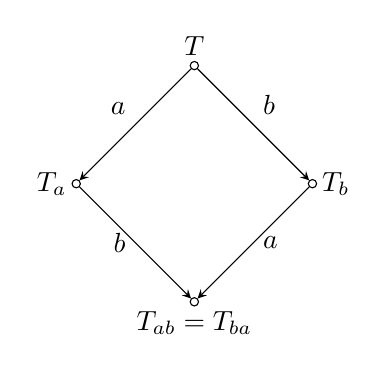
\begin{tikzpicture}[>=stealth]
    % nodes
    \node[circle,draw,inner sep=1pt,minimum size=3pt] (T)   at (0,0)    {};
    \node[circle,draw,inner sep=1pt,minimum size=3pt] (Ta)  at (-1.5,-1.5) {};
    \node[circle,draw,inner sep=1pt,minimum size=3pt] (Tb)  at (1.5,-1.5)  {};
    \node[circle,draw,inner sep=1pt,minimum size=3pt] (Tab) at (0,-3)   {};

    % labels
    \node[above] at (T)   {$T$};
    \node[left]  at (Ta)  {$T_a$};
    \node[right] at (Tb)  {$T_b$};
    \node[below] at (Tab) {$T_{ab}=T_{ba}$};

    % arrows
    \draw[->] (T)  -- node[above left]  {$a$} (Ta);
    \draw[->] (T)  -- node[above right] {$b$} (Tb);
    \draw[->] (Ta) -- node[left]        {$b$} (Tab);
    \draw[->] (Tb) -- node[right]       {$a$} (Tab);
  \end{tikzpicture}
  \caption{Local diamond for commuting disjoint updates. Starting from a common
  state $T$, two spacelike-separated reductions $a$ and $b$ can be applied in
  either order, yielding intermediate states $T_a$ and $T_b$ but the same final
  state $T_{ab}=T_{ba}$. The two intermediate events are spacelike-separated:
  they share a common past ($T$) and a common future ($T_{ab}$) but no causal edge
  between them. This expresses a microcausality analogue on the Catalan substrate:
  local updates supported on disjoint subtrees commute and differ only by temporal
  ordering.}
  \label{fig:disjoint-subtrees}
\end{figure}

(See Appendix~\ref{appendix:computational-foundations}, and in particular
Lemma~\ref{lem:causal-consistency}, for a formal statement and proof sketch
of the corresponding disjoint-commutation property.)

\subsection{Collapse and selection}
Both computation and amplitude propagation require selection:
\begin{itemize}
	\item computational reduction chooses a redex,
	\item measurement-like selection chooses an observable outcome, corresponding
		to an equivalence class under the chosen projection.
\end{itemize}
In the Catalan substrate, selection operates locally, refining rather than
destroying structure. The global constraint ensures consistency after
selection. The formal development of collapse probabilities lies beyond the
scope of this paper and is treated here only structurally.

\subsection{Summary}
Locality and disjoint commutation emerge directly from the causal and recursive
structure of the Catalan lattice. The same principles underlie both
computational reduction and quantum amplitude constructions on the Catalan
history space.

\section{Discussion and Limitations}
\label{sec:discussion}

The results presented here establish a shared structural basis for causal
geometry, quantum dynamics, and computation. Several limitations should be
emphasized:
	\begin{itemize}
		\item Physical constants and interactions are not derived.
		\item Only free (noninteracting) wave dynamics appears explicitly.
		\item Collapse probabilities are not fixed uniquely by the structure.
		\item Lorentz symmetry is discussed only via continuum embeddings; no discrete
			boost invariance is claimed.
		\item The choice of phase/action functional (e.g.\ Dyck area) is not shown to
			be unique.
	\end{itemize}
These limitations reflect a deliberate restriction of scope. The goal has been
to isolate the minimal recursive structure common to multiple domains, not to
provide a complete physical theory.

\subsection{Relation to discrete quantum gravity}

Similar scaling behavior appears in two-dimensional quantum gravity and random
surface models. In particular, Causal Dynamical Triangulations (CDT) enforce a
preferred foliation and causal constraint that parallels the prefix order of
Dyck paths \cite{ambjorn01,ambjorn12}. In CDT, the continuum limit is taken
after summing over causally admissible triangulations. Here the admissible
structures are Dyck paths rather than triangulations, but the organizing
principle---the restriction to histories that respect a causal growth rule---is
closely analogous.

\section{Conclusion}
\label{sec:conclusion}

This paper treats the Catalan family---Dyck paths, full binary trees, and
balanced-parenthesis expressions---as a single discrete history space supporting
three complementary readings: causal geometry via the prefix order, computation
via application trees and local rewrites, and amplitudes via coherent summation
over coarse-grained outcomes. Classical scaling results for conditioned walks
provide a continuum comparison in which Dyck ensembles converge to Brownian
excursions and the diffusion limit is governed by the heat operator on the
half-line; under analytic continuation one obtains the free Schr\"odinger
equation. The scope is intentionally restricted to this shared structural core:
deriving interactions, constants, or a unique collapse/measurement rule requires
additional structure beyond what is developed here.

\appendix

\section{Coordinate Charts and Continuum Comparisons}
\label{appendix:coordinate-charts}

This appendix collects optional coordinate embeddings and continuum comparisons
used for intuition; the combinatorial results in the main text do not depend on
these constructions.

\subsection{Coordinate charts on the Catalan cone}
\label{sec:coordinate-charts}

\begin{remark}[Notation hygiene]
\label{rem:notation-hygiene}
To avoid collisions, the \emph{tier} (semilength) of a completed history is
denoted by $n$. A \emph{prefix length} is denoted by $k\in\{0,1,\dots,2n\}$.
Within this subsection only, the symbols $(t_k,x_k)$ denote an \emph{embedded}
spacetime chart derived from cumulative counts (Definition~\ref{def:null-counts}),
and should not be confused with the tier index $n$ used elsewhere.
\end{remark}

\paragraph{The Catalan cone as the master object.}
Let $\mathcal{C}$ denote the set of Dyck prefixes (balanced-parentheses
\emph{prefixes} that never go below height $0$), partially ordered by extension:
$p\preceq q$ iff $q$ has prefix $p$. A completed history is a maximal element
$w\in\mathcal{D}_n\subset\mathcal{C}$ of semilength $n$.
For any prefix $p\in\mathcal{C}$, the future
\[
\mathcal{C}(p)\;:=\;\{\,q\in\mathcal{C}: p\preceq q\,\}
\]
is canonically a ``local cone'' rooted at $p$: the same growth law, re-centered.
Thus there is a single substrate $\mathcal{C}$ (and its re-rootings), and
different ``cones'' arise from different coordinate charts or coarse-grainings
of this same object.

\paragraph{Two cumulative counts and a light-cone chart.}
The most rigid chart on $\mathcal{C}$ is obtained by tracking the cumulative
numbers of opens and closes.

\begin{definition}[Null counts and embedded coordinates]
\label{def:null-counts}
Fix a Dyck word $w\in\mathcal{D}_n$, and let $w[1\!:\!k]$ denote its length-$k$
prefix. Define
\[
u(k)\;:=\;\#\{\texttt{(}\text{ in }w[1\!:\!k]\},\qquad
v(k)\;:=\;\#\{\texttt{)}\text{ in }w[1\!:\!k]\}.
\]
The Dyck admissibility constraint is $u(k)\ge v(k)$ for all $k$, and completion
is $u(2n)=v(2n)=n$. Define the height (frontier) process
\[
H(k)\;:=\;u(k)-v(k)\;\ge\;0,
\]
and the embedded ``spacetime'' coordinates
\[
t_k\;:=\;\frac{u(k)+v(k)}{2}\;=\;\frac{k}{2},\qquad
x_k\;:=\;\frac{u(k)-v(k)}{2}\;=\;\frac{H(k)}{2}.
\]
Equivalently $u=t_k+x_k$ and $v=t_k-x_k$ (a discrete null-coordinate form).
\end{definition}

Under this embedding, each symbol advances time and changes space by one unit
(up to the $1/2$ normalization):
\[
\texttt{(}:\ (t,x)\mapsto (t+\tfrac12,\ x+\tfrac12),\qquad
\texttt{)}:\ (t,x)\mapsto (t+\tfrac12,\ x-\tfrac12).
\]
Hence the path stays inside the cone $|x_k|\le t_k$, with the boundary $x_k=0$
representing zero frontier (no outstanding opens).

\paragraph{Why ``return to $0$'' is not ``return to the origin.''}
The completion constraint $H(2n)=0$ means only that the \emph{imbalance} vanishes:
every open has been matched by a close. In spacetime coordinates, the endpoint is
\[
(t_{2n},x_{2n})\;=\;\bigl(n,0\bigr),
\]
not $(0,0)$. Thus a history expands monotonically in $t$ (prefix length grows),
while the spatial coordinate $x$ is a \emph{frontier variable} that eventually
returns to $0$ because no unfinished structure may remain at completion.

\paragraph{Pairs, trees, and $S$-expressions are identical structure.}
A Dyck word $w$ can be read as a parenthesized $S$-expression skeleton, and it
already \emph{is} a rooted ordered tree:
matched parenthesis pairs are nodes; containment defines parent/child; and
left-to-right order in the string gives sibling order.
For example, $w=\texttt{(()())}$ has one outer pair (the root) containing two
inner pairs (two leaves). Under this identification, the height $H(k)$ is the
number of currently-open pairs---the size of the \emph{active frontier} of the
tree under construction.

\paragraph{Evaluation ``return'' as frontier discharge.}
If evaluation is recorded at the level of control (continuations), then entering
a subproblem pushes a context frame and finishing it pops that frame. In a
well-bracketed evaluation regime, this push/pop trace is Dyck, and the same
counts $(u(k),v(k))$ track control events. The embedded coordinate $x_k$
therefore measures continuation depth (pending contexts), and the return to
$x=0$ at termination is the emptying of the continuation stack: no pending
contexts remain. Value return is mediated by this control return; the Dyck
``return'' is fundamentally the discharge of outstanding obligations.

\paragraph{Breadth as a different projection (history-level, not frontier-level).}
Statistics such as breadth $r(w)$ summarize a \emph{completed} history by the
maximum size of a constant-depth slice in its associated tree. This is a
coarse-graining of $w$ (many distinct histories share the same $(n,r)$), and it
should be distinguished from the frontier coordinate $x_k$, which is an
instantaneous depth/obligation variable along a single prefix trajectory.

\paragraph{Summary of the two readings.}
There is one substrate $\mathcal{C}$ (and its re-rooted futures $\mathcal{C}(p)$).
Two useful ``cone'' pictures arise from:
(i) the embedded prefix trajectory $(t_k,x_k)$ derived from null counts
(pathwise frontier dynamics), and
(ii) history-level projections such as $(n,r(w))$ (coarse geometric envelope).
The pairs/tree/$S$-expression view does not introduce a new object; it is an
identity of representations of the same Catalan structure.

\subsection{Dyck Coordinates, Lorentz Geometry, and Computational Proper Time}
\label{subsec:dyck-lorentz-computation}

\begin{remark}[Indices and coordinate conventions]
Throughout, $n$ denotes the tier (semilength) of a completed Dyck history.
Within this subsection, $k\in\{0,1,\dots,2n\}$ denotes a \emph{step index} along a
single history, and $m$ denotes the number of \emph{collapse events} (local redex
contractions) performed by a chosen evaluation strategy.
\end{remark}

A Dyck history $w\in\mathcal D_n$ induces the height process $H(k)$ of
Definition~\ref{def:null-counts}. The corresponding embedded coordinates are
$t_k=k/2$ and $x_k=H(k)/2$, so that each parenthesis advances time by $\tfrac12$
and changes the transverse coordinate by $\pm\tfrac12$:
\[
\texttt{(}:\ (t,x)\mapsto (t+\tfrac12,\ x+\tfrac12),\qquad
\texttt{)}:\ (t,x)\mapsto (t+\tfrac12,\ x-\tfrac12).
\]
For any walk with steps $(\Delta t,\Delta x)=(\tfrac12,\pm\tfrac12)$ one has the
kinematic cone bound $|x_k-x_0|\le t_k-t_0$. In the Dyck case, the additional
constraint is one-sided: $x_k\ge 0$ for all $k$, together with the endpoint
condition $x_{2n}=0$. Thus Dyck histories occupy the right half of a discrete
light cone and return to the axis only at completion.

Introduce discrete null coordinates (compare Definition~\ref{def:null-counts})
\[
u:=t+x,\qquad v:=t-x.
\]
In continuum $(1+1)$-dimensional Minkowski space, a Lorentz boost with rapidity
$\eta$ acts linearly as
\begin{equation}
u' = e^{\eta} u,\qquad v' = e^{-\eta} v,
\label{eq:lightcone-boost}
\end{equation}
and transforming back to $(t,x)$ yields the standard Lorentz transformation
\begin{equation}
t' = \gamma (t - v_{\!L} x),\qquad x' = \gamma (x - v_{\!L} t),
\label{eq:lorentz-tx}
\end{equation}
where
\[
\gamma=\frac{1}{\sqrt{1-v_{\!L}^2}},\qquad v_{\!L}=\tanh\eta,
\]
in units $c=1$. The Minkowski interval
\begin{equation}
\mathrm{d}s^{2}=\mathrm{d}t^{2}-\mathrm{d}x^{2}
\label{eq:minkowski}
\end{equation}
is invariant under~\eqref{eq:lorentz-tx}. In this sense the step rule supplies a
discrete null-step kinematics, while the Dyck constraint supplies the boundary
and return conditions selecting the Catalan ensemble. We emphasize that generic
nontrivial boosts do not preserve the discrete Dyck lattice itself (the counts
$u,v$ are integers), so the Lorentz discussion here is a continuum comparison
for the embedded coordinates rather than a discrete symmetry claim.

\paragraph{Computational proper time.}
A reduction history carries an intrinsic progress parameter given by the count
of collapse events. Let $m$ be the number of local redex contractions performed
by an evaluation strategy up to a given stage, and define the \emph{computational
proper time}
\begin{equation}
\tau := \alpha\, m,
\label{eq:tau-discrete}
\end{equation}
where $\alpha>0$ is the characteristic scale associated with a single collapse.
In continuum Minkowski space, a parametrized world-line $(t(s),x(s))$ admits a
proper-time functional
\begin{equation}
\left(\frac{\mathrm{d}\tau}{\mathrm{d}s}\right)^{2}
=
\left(\frac{\mathrm{d}t}{\mathrm{d}s}\right)^{2}
-
\left(\frac{\mathrm{d}x}{\mathrm{d}s}\right)^{2},
\label{eq:proper-time-continuum}
\end{equation}
which is Lorentz-invariant under~\eqref{eq:lorentz-tx}. In the present discrete
setting, Equation~\eqref{eq:tau-discrete} is simply a well-defined event-count
parameter; the analogy is that collapse count plays the role of a proper-time
progress variable along a chosen computational history.

\subsection{Projection to Height Dynamics and Correlation Structure}
\label{subsec:projection-correlation}

Let $\mathcal{C}$ denote the set of Dyck prefixes, i.e.\ finite words in
$\{(,)\}$ whose height never falls below zero. Each prefix
$p \in \mathcal{C}$ has an associated height
$h(p) \in \mathbb Z_{\ge 0}$ given by the net excess of opening over closing
parentheses. Completed Dyck words of semilength $n$ form the subset
$\mathcal D_n \subset \mathcal{C}$ of prefixes of length $2n$ with
$h=0$.

The Catalan growth rule specifies admissible extensions: from a prefix $p$,
one may append ``$(\,$'' unconditionally, or ``$)\,$'' provided $h(p)>0$.
To describe this probabilistically, it is convenient to separate the base
process from the Dyck-conditioned ensemble.

\paragraph{Base height process.}
Let $(H_t)_{t\ge0}$ be a simple symmetric random walk on $\mathbb Z$ with
increments $\pm1$. This walk is time-homogeneous and Markov. Its sample paths
may be viewed as unconstrained height sequences, without regard to the Dyck
condition.

\paragraph{Dyck conditioning.}
The Dyck ensemble of length $T=2n$ is obtained by conditioning the base walk on
the event
\[
\{ H_t \ge 0 \text{ for all } t \le T,\; H_T = 0 \}.
\]
Under this conditioning, the law of $(H_t)_{t=0}^T$ is uniform on Dyck paths of
semilength $n$. Equivalently, the conditioned process may be represented via a
Doob $h$-transform (or bridge kernel) of the base walk. In this representation,
the height process remains Markov but becomes time-inhomogeneous due to the
global conditioning. Each completed Dyck word
$p \in \mathcal D_n$ corresponds uniquely to a sample path
\[
(h_0,h_1,\dots,h_T), \qquad h_0=h_T=0,\; h_t\ge0,
\]
drawn from this conditioned law.

\paragraph{Correlation structure.}
Consider the ensemble of height paths of fixed length $T$, distributed
according to the Dyck-conditioned law. Define the mean and covariance functions
\[
\mu_t := \mathbb E[H_t], \qquad
C(s,t) := \mathbb E\!\left[(H_s-\mu_s)(H_t-\mu_t)\right],
\qquad 0\le s,t\le T .
\]
The covariance kernel $C$ is a symmetric positive operator on the finite-dimensional
space $\mathbb R^{T+1}$ and captures the second-order temporal structure induced
by the Dyck constraint. It admits an eigen-decomposition
\[
\sum_{t=0}^{T} C(s,t)\,v^{(k)}_t = \lambda_k\, v^{(k)}_s ,
\]
yielding an orthogonal family of temporal modes. Any centered height profile
admits the expansion
\[
H_t-\mu_t = \sum_k \xi_k\, v^{(k)}_t ,
\qquad \mathbb E[\xi_k\xi_\ell]=\lambda_k\,\delta_{k\ell}.
\]
In this precise sense, the eigenvalues $\lambda_k$ constitute the spectrum of
temporal correlations induced by the Dyck-conditioned dynamics, and the
associated eigenvectors provide a canonical modal decomposition
(Karhunen--Lo\`eve expansion) of Dyck height signals.

\paragraph{Scaling limit.}
Under diffusive scaling, the base random walk converges to Brownian motion on
$\mathbb R$. The Dyck-conditioned law converges to Brownian excursion, which may
be described equivalently as Brownian motion conditioned to remain nonnegative
and return to zero, or via a Doob transform / Bessel-bridge representation
\cite{takacs1991,pitman1999}. The resulting continuum evolution is governed by a
second-order differential operator on $\mathbb R_{\ge0}$ whose drift and boundary
behavior encode the conditioning. In related unconditioned or bridge settings,
the associated covariance eigenfunctions are explicitly sinusoidal; for the
excursion case, the exact eigenstructure is more subtle, though the dominant
modes often resemble sine-like functions away from boundaries.

Thus, the appearance of modal structure follows directly from the projection of
Catalan growth dynamics to the height observable and the standard spectral
analysis of the resulting correlation kernel, without the introduction of
additional physical assumptions.

\begin{remark}[Self-similarity and reference frames]
The Dyck prefix structure is recursively self-similar: every prefix is itself
the root of a complete Catalan subtree. Consequently, distinctions such as
parent and child, past and future, or global and local history are not
intrinsic to the substrate but arise only after fixing a reference root, which
induces a causal orientation. The projected height dynamics, their conditioning,
and their scaling limits are invariant under such re-rootings.
\end{remark}

\section{Additional Technical Notes}
\label{appendix:technical-notes}

\subsection{Entropy of coarse-graining and information rate}

Fix a tier $n$ and an observable (deterministic coarse-graining)
$f:\mathcal D_n\to\mathcal X$. For $x\in\mathcal X$ write
\[
N(x)\;:=\;\#\{w\in \mathcal D_n: f(w)=x\},
\]
so that $f^{-1}(x)$ is the equivalence class of histories identified as the
same outcome.

\paragraph{Multiplicity entropy.}
Define the (microcanonical) entropy of the full ensemble at tier $n$ by
\[
S_n \;:=\; \log \#(\mathcal D_n),
\]
and the conditional entropy of an outcome $x$ by
\[
S(x) \;:=\; \log N(x).
\]
The information eliminated by selecting outcome $x$ is the entropy drop
\[
\Delta S(x)\;:=\; S_n - S(x)
\;=\; \log\!\Big(\frac{\#(\mathcal D_n)}{N(x)}\Big).
\]
(Any logarithm base may be used; base $2$ yields units of bits.)

\begin{remark}[Retrospective vs.\ prospective counts]
The multiplicity entropy $S(x)=\log N(x)$ measures how many fine-grained
histories are identified as the same outcome at tier $n$. A complementary
forward-looking quantity is the number of admissible continuations of a
realized prefix into higher tiers (the size of its local cone; see
Section~\ref{sec:multiplecones}), which may be studied by analogous counting of
completions.
\end{remark}

\paragraph{Information rate as rate of possibility reduction.}
Let $m$ denote the number of selection events (local contractions) along a
history, and let computational proper time be $\tau=\tau_0 m$ for a fixed scale
$\tau_0>0$. We define the information rate associated with outcome $x$ to be the
information loss per unit computational proper time,
\[
R(x)\;:=\;\frac{\Delta S(x)}{\tau}.
\]
In the simplest case of a single event ($m=1$), this reduces to
$R(x)=\Delta S(x)/\tau_0$.
One may also adopt a coarser tier-wise selection model in which $m$ is
identified with the tier index $n$ (one selection per tier boundary), but we
keep these notions separate in general.

\paragraph{Gauge-invariant counting.}
When histories admit a redundancy under commuting spacelike-separated updates,
one may quotient $\mathcal D_n$ by the induced gauge equivalence relation
$\sim_g$ and define $\bar{\mathcal D}_n:=\mathcal D_n/\!\sim_g$. If $f$ is
gauge-invariant (constant on $\sim_g$-orbits), define
\[
\bar N(x):=\#\{[w]\in \bar{\mathcal D}_n : f(w)=x\},
\qquad
\bar{\Delta S}(x):=\log\!\Big(\frac{\#(\bar{\mathcal D}_n)}{\bar N(x)}\Big),
\]
and use $\bar{\Delta S}$ in place of $\Delta S$. This removes overcounting due
solely to reordering of independent collapses.

\section{A Double-Slit Thought Experiment on the Catalan Light Cone}
\label{appendix:doubleslit}

This appendix provides an illustrative thought experiment showing how the
discrete path-integral formalism developed in Section~\ref{sec:amplitudes}
exhibits interference in a setting analogous to the double-slit experiment.
The construction is entirely combinatorial and finite. No new assumptions,
dynamical rules, or continuum limits are introduced; the purpose is solely to
instantiate the formalism in a familiar narrative.
Throughout, we take the phase functional to be the Dyck area $A(w)$ introduced
in Section~\ref{sec:amplitudes}, i.e.\ $\psi(w)=e^{i\alpha A(w)}$ (a special
case of Proposition~\ref{prop:phase-classification}).

\subsection{Two sources as boundary-conditioned cones}

Consider two distinct Dyck prefixes $u_L$ and $u_R$ of equal length and height.
Each prefix induces a local Catalan cone of admissible continuations, as
described in Section~\ref{sec:multiplecones}. We refer to these as the left and
right source cones, although no spatial interpretation is assumed at this
stage.

Both cones are evolved to a common tier $n$, producing two ensembles of Dyck
paths of semilength $n$ that differ only in their initial boundary condition.
The admissible histories from both cones are evaluated relative to the same
observable defined below.

\subsection{Observable and indistinguishability}

Fix a tier $n$ and define an observable
\[
f : \mathcal D_n \to \mathcal X,
\]
where $\mathcal X$ is a discrete outcome space. The observable $f$ retains a
coarse-grained feature of each history (for example, a bin determined by the
mean height or total area) and discards all other information, including which
source cone the history originated from.

Interference arises precisely because histories originating from distinct cones
may be rendered indistinguishable by the observable. If the observable were to
retain source information, no interference would occur.

\subsection{A worked finite example}
\label{subsec:doubleslit-worked}

Take $n=4$ and choose two admissible Dyck prefixes of equal length and height,
\[
u_L=\texttt{(()(}, \qquad u_R=\texttt{()((},
\]
each of length $4$ and height $2$. Each prefix admits exactly three completions
to a full Dyck word of length $8$, yielding six histories in the union of the
two source cones.

Define a coarse observable that discards source information by sampling the
height at a fixed time step after the ``slits'':
\[
f(w) := H_w(6)\in\{0,2\}.
\]
This is a discrete analogue of recording transverse displacement at a detector
time without access to which slit was taken.

\begin{table}[h]
\centering
\begin{tabular}{llll}
\hline
cone & $w$ & $A(w)$ & $f(w)=H_w(6)$ \\
\hline
$L$ & \texttt{(()(()))} & $12$ & $2$ \\
$L$ & \texttt{(()()())} & $10$ & $2$ \\
$L$ & \texttt{(()())()} & $8$  & $0$ \\
$R$ & \texttt{()((()))} & $10$ & $2$ \\
$R$ & \texttt{()(()())} & $8$  & $2$ \\
$R$ & \texttt{()(())()} & $6$  & $0$ \\
\hline
\end{tabular}
\caption{Two equal-height source cones at $n=4$ and a coarse detector observable.}
\end{table}

With phase $\psi(w)=e^{i\alpha A(w)}$, the detector amplitudes are
\[
\Psi(2)=\sum_{f(w)=2} e^{i\alpha A(w)}
= e^{i12\alpha}+2e^{i10\alpha}+e^{i8\alpha}
= 2e^{i10\alpha}\bigl(1+\cos(2\alpha)\bigr),
\]
\[
\Psi(0)=\sum_{f(w)=0} e^{i\alpha A(w)}
= e^{i8\alpha}+e^{i6\alpha}
= 2e^{i7\alpha}\cos(\alpha).
\]
Classically one would predict multiplicities $N(2)=4$ and $N(0)=2$. In contrast,
the quantum intensities $|\Psi(x)|^2$ vary with $\alpha$ and can exhibit strong
suppression. For example, at $\alpha=\pi/2$ one obtains $\Psi(2)=0$ (exact
destructive interference at the outcome $x=2$), even though $N(2)=4$ histories
contribute.

This example is intentionally tiny: its purpose is to show, in finite
combinatorial terms, how (i) multiple histories per outcome, (ii) an additive
phase functional, and (iii) coarse observation together produce interference.
Larger $n$ yields richer outcome sets and more intricate cancellation patterns.

\subsection{Summary}
No wave equation, spatial geometry, or continuum approximation is assumed in
this construction. The example simply instantiates the general mechanism of
Section~\ref{sec:amplitudes}: complex weights, coherent summation over
coarse-grained preimages, and Born-style squaring suffice to produce
interference.

\section{Computational Foundations}
\label{appendix:computational-foundations}

This appendix records proof sketches for the computational claims used in the
main text, including Proposition~\ref{prop:catalan-programs} and the
disjoint-commutation property of Lemma~\ref{lem:causal-consistency}. For a lean
v1, extended examples and additional formal development are omitted.

\begin{lemma}[Internalizing Symbols as Motifs]
\label{lem:symbol-motifs}
Let $\Sigma$ be a finite (or countable) alphabet of atomic symbols, and consider
finite applicative terms over $\Sigma$ (binary application with atoms). There
is an injective encoding of such labeled application trees into the Catalan
family $\mathcal{C}$ of unlabeled full binary trees. One explicit construction
fixes two distinct tag trees $A,B\in\mathcal{C}$, assigns each
$\sigma\in\Sigma$ a distinct motif $S_\sigma\in\mathcal{C}\setminus\{A,B\}$, and
defines
\[
	E(\sigma)\;:=\;\bullet(A,S_\sigma),\qquad
	E(t\cdot u)\;:=\;\bullet\bigl(B,\bullet(E(t),E(u))\bigr),
\]
where $t\cdot u$ denotes application and $\bullet(\,\cdot\,,\,\cdot\,)$ denotes
binary pairing of subtrees. The left tag distinguishes atoms from applications,
so $E$ is recursively decodable and therefore injective.
\end{lemma}


\begin{proof}[Proof Sketch (of Proposition~\ref{prop:catalan-programs})]
			As described in classical treatments of combinatory logic and the
			$\lambda$-calculus \cite{CurryFeys1958,barendregt84}, application is a
		binary operation, and every term therefore possesses a unique representation
		as a full binary tree: internal nodes encode application, and leaves encode
	variables, constants, or combinators.  This establishes a canonical embedding
	of programs into $\mathcal{C}$.

	Conversely, any full binary tree with labeled leaves may be interpreted as a
	well-formed program term by reading internal nodes as applications and leaves
	as atomic symbols, yielding a unique term up to $\alpha$-equivalence.

	Operational semantics are defined via local tree rewrites.  A $\beta$-redex
	$(\lambda x.M)\,N$ contracts by replacing the parent application with
	$M[x:=N]$; SKI reductions replace specific subtrees according to fixed
	patterns.  In each case, the output remains a full binary tree, so evaluation
	never leaves $\mathcal{C}$.  Because nondeterministic redex choices correspond
	to branching in the space of trees, each complete reduction sequence is a path
	through the Catalan possibility space, completing the correspondence.
\end{proof}


\begin{lemma}[Commutation of disjoint reductions]
	\label{lem:causal-consistency}
	Let $T$ be a full binary tree and consider any local rewrite system whose
	single-step reductions replace a rooted subtree matching a finite pattern by a
	new subtree, leaving the rest of $T$ unchanged. Suppose two single-step
	reductions are applicable at positions $p$ and $q$ whose rooted subtrees are
	disjoint (neither position lies on the root-to-node path of the other). Let
	$T_p$ denote the result of applying the reduction at $p$, and similarly $T_q$.
	Then both reductions remain applicable after the other, and they commute:
	\[
		(T_p)_q \;\equiv\; (T_q)_p.
	\]
	In particular, disjoint reductions form a commuting diamond as in
	Figure~\ref{fig:disjoint-subtrees}.
\end{lemma}

\begin{proof}[Proof Sketch]
	Since $p$ and $q$ lie in disjoint subtrees, contracting at $p$ rewrites only
	the subtree rooted at $p$ and leaves the subtree rooted at $q$ unchanged.
	Symmetrically, contracting at $q$ leaves the subtree at $p$ unchanged. Because
	the two rewrite steps act on disjoint parts of the tree, performing both
	contractions yields the same result regardless of order.
\end{proof}

		\bibliographystyle{plain}
		\begin{thebibliography}{99}

	\bibitem{addario-berry13}
	L.~Addario-Berry, L.~Devroye, and S.~Janson.
	\newblock Sub-Gaussian tail bounds for the width and height of conditioned
	Galton--Watson trees.
	\newblock {\em Annals of Probability}, 41(2):1074--1087, 2013.

	\bibitem{ambjorn01}
	J.~Ambj{\o}rn, J.~Jurkiewicz, and R.~Loll.
	\newblock Dynamically triangulating Lorentzian quantum gravity.
	\newblock {\em Nuclear Physics B}, 610:347--382, 2001.

	\bibitem{ambjorn12}
	J.~Ambj{\o}rn, A.~G{\"o}rlich, J.~Jurkiewicz, and R.~Loll.
	\newblock Nonperturbative quantum gravity.
	\newblock {\em Physics Reports}, 519:127--210, 2012.

	\bibitem{barendregt84}
	H.~P. Barendregt.
	\newblock {\em The Lambda Calculus: Its Syntax and Semantics}.
	\newblock North-Holland, 1984.

	\bibitem{bombelli87}
	L.~Bombelli, J.~Lee, D.~Meyer, and R.~D. Sorkin.
	\newblock Space-time as a causal set.
	\newblock {\em Physical Review Letters}, 59(5):521--524, 1987.

	\bibitem{church33}
	A.~Church.
	\newblock A set of postulates for the foundation of logic.
	\newblock {\em Annals of Mathematics}, 34:839--864, 1933.

	\bibitem{cover-thomas}
	T.~M. Cover and J.~A. Thomas.
	\newblock {\em Elements of Information Theory}.
	\newblock 2nd edition, John Wiley \& Sons, 2006.

		\bibitem{CurryFeys1958}
		H.~B. Curry and R.~Feys.
		\newblock {\em Combinatory Logic, Vol.~I}.
		\newblock North-Holland, 1958.

	\bibitem{feynman-hibbs65}
	R.~P. Feynman and A.~R. Hibbs.
	\newblock {\em Quantum Mechanics and Path Integrals}.
	\newblock McGraw--Hill, 1965. (Dover reprint, 2010).

	\bibitem{janson07}
	S.~Janson.
	\newblock Brownian excursion area, Wright's constants in graph enumeration, and
	other Brownian areas.
	\newblock {\em Probability Surveys}, 4:80--145, 2007.

	\bibitem{kac49}
	M.~Kac.
	\newblock On distributions of certain Wiener functionals.
	\newblock {\em Transactions of the American Mathematical Society},
	65(1):1--13, 1949.

	\bibitem{le-gall05}
	J.-F. Le~Gall.
	\newblock Random trees and applications.
	\newblock {\em Probability Surveys}, 2:245--311, 2005.

		\bibitem{orus14}
		R.~Or\'us.
			\newblock A practical introduction to tensor networks: Matrix product states and
			projected entangled pair states.
			\newblock {\em Annals of Physics}, 349:117--158, 2014.

		\bibitem{pitman1999}
		J.~Pitman.
		\newblock Brownian motion, bridge, excursion, and meander revisited.
		\newblock {\em Electronic Journal of Probability}, 4:1--32, 1999.

		\bibitem{rovelli04}
		C.~Rovelli.
		\newblock {\em Quantum Gravity}.
		\newblock Cambridge University Press, 2004.

			\bibitem{stanley-catalan}
			R.~P. Stanley.
			\newblock {\em Catalan Numbers}.
			\newblock Cambridge University Press, 2015.

		\bibitem{takacs1991}
		L.~Tak{\'a}cs.
		\newblock A {B}ernoulli excursion and its various applications.
		\newblock {\em Advances in Applied Probability}, 23(3):557--585, 1991.

	\end{thebibliography}
\end{document}
